
As discussed in \cref{cache-impl}, to accelerate the computation of upward and downward covers, a cache was implemented to avoid repeated calls to the reasoner, when the necessary information can already be inferred from previous computations. This section will discuss the experiments performed to evaluate the effectiveness of the cache implementation.

Three versions of the upward and downward cover have been considered, the uncached version that calls the reasoner for every subsumption query, a version that caches only the exact queries that were already made previously, and finally the version that additionally infers some additional information from the transitivity of subsumption as listed in \cref{algo:cached-subs}. The experiment uses some of the same ontologies as have been used for the previously discussed evaluation of the repair quality. From the logical axioms of each ontology were selected, uniformly at random, one hundred groups with a fixed number of axioms. The same axioms may be selected multiple times. Each of the groups was then tested with a separate instance of the cache. The rationale behind testing with different group sizes is that the cache will obviously have a greater impact when the same cache can be reused for more cover computations. In each test run, the axiom weakening operator was applied to each axiom and the number of reasoner calls and (real) time taken were measured. The weakening operator used the complete (after post-processing) ontology as the reference ontology. The test has further been performed using different OWL 2 DL reasoners. The final results of the evaluation can be seen in table \cref{table:results-cache-calls} and are visualized in figure \cref{fig:results-cache-calls}. Note that a logarithmic y-axis has been used in the bar plots.

\begin{table}[ht]
  \scriptsize
  \centering
  \begin{tabular}{|l|rrr|rrr|rrr|}
    \cline{2-10}
    \multicolumn{1}{l|}{} & \multicolumn{9}{c|}{\hspace{-4mm}Reasoner calls per weakening} \\
    \multicolumn{1}{l|}{} & \multicolumn{3}{c}{Full caching} & \multicolumn{3}{c}{Simple caching} & \multicolumn{3}{c|}{No caching} \\
    \multicolumn{1}{l|}{} & \multicolumn{1}{c}{1} & \multicolumn{1}{c}{10} & \multicolumn{1}{c}{100} & \multicolumn{1}{c}{1} & \multicolumn{1}{c}{10} & \multicolumn{1}{c}{100} & \multicolumn{1}{c}{1} & \multicolumn{1}{c}{10} & 100 \\
    \hline
    admin & 1096 & 222 & 35
      & 15138 & 2115 & 236
      & 41105 & 41288 & 41751 \\
    cdpeo & 2110 & 522 & 75
      & 13621 & 2694 & 312
      & 29051 & 28617 & 29315 \\
    emo & 2652 & 1355 & 258
      & 7781 & 2784 & 619
      & 12524 & 12134 & 12552 \\
    gbm & 3019 & 1074 & 168
      & 12572 & 3284 & 503
      & 19490 & 21330 & 20801 \\
    gfvo & 1737 & 575 & 80
      & 2828 & 1524 & 293
      & 4058 & 4104 & 4003 \\
    koro & 2006 & 591 & 80
      & 5154 & 2272 & 382
      & 7271 & 7181 & 7422 \\
    mamo &  1984 & 511 & 61
      & 3557 & 1488 & 234
      & 5060 & 5059 & 4998 \\
    \hline
    Overall & 2086 & 693 & 108
      & 8664 & 2309 & 368
      & 16937 & 17102 & 17263 \\
    \hline
  \end{tabular}
  \caption{Results of the evaluation of cache effectiveness. The mean number of reasoner calls required for a single weakening is given for one, ten, and one hundred applications of the operator using the same cache.}
  \label{table:results-cache-calls}
\end{table}

\begin{figure}[ht]
  \centering
  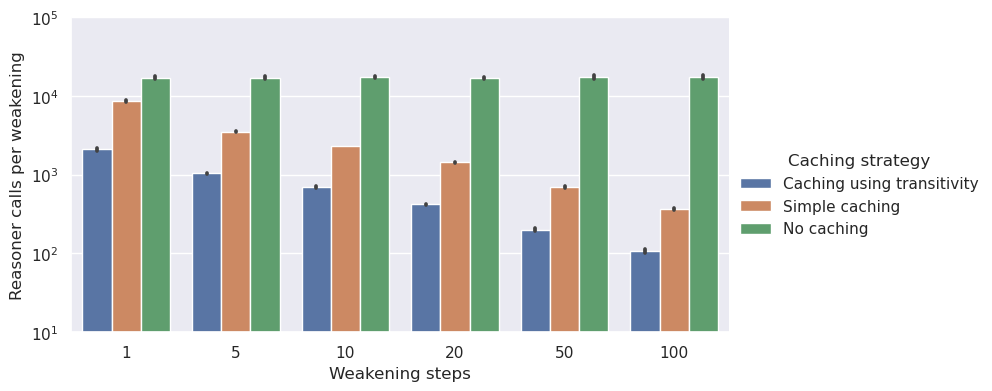
\includegraphics[width=\textwidth]{resources/calls-cache-bar.png}
  \caption{The mean number of reasoner calls needed for a single application of the axiom weakening operator, averaged over the tested ontologies.}
  \label{fig:results-cache-calls}
\end{figure}

\begin{figure}[ht]
  \centering
  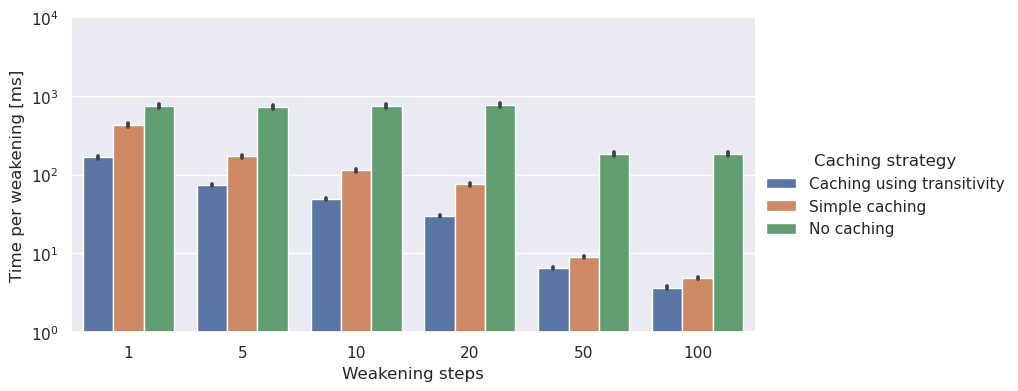
\includegraphics[width=\textwidth]{resources/time-cache-bar.png}
  \caption{Average time required per application of the axiom weakening operator with different caching strategies when executing axiom weakening of random axioms. The results are averaged over the tested ontologies and the reasoners FaCT++, JFact, Openllet, and HermiT.}
  \label{fig:results-cache-time}
\end{figure}

We can see clearly from the results that the cache is indeed effective at lowering both the number of reasoner calls and execution time. The simple caching method alone provides a dramatic decrease in the number of reasoner calls, especially at higher group sizes. The algorithm that can additionally exploit the transitivity of the relation performs even better, also with a smaller number of weakening steps. The difference when looking at the execution time is significantly smaller. This can likely be attributed largely to internal caching performed by the reasoners. This would also explain the observed variation when it comes to the relative improvement between different reasoners. It can be concluded that the addition of the cache greatly benefits the computation of the axiom weakening operator, especially if it can be reused for many applications of the same weakening operator.

